\documentclass[../main.tex]{subfiles}

\makeatletter
\@ifundefined{fromRoot}{%
  \newcommand{\fromRoot}[1]{../#1}
  
  \usepackage{xr}
  \externaldocument{../main}
}{}

\def\input@path{{\subfix{../}}}
%or: \def\input@path{{/path/to/folder/}{/path/to/other/folder/}}
\makeatother

\graphicspath{
  {\subfix{../}}
  {\subfix{./figures}}
  {\subfix{../figures}}
  {\subfix{./figures/logos-thesis/}}
  {\subfix{../figures/logos-thesis/}}
  {\subfix{./figures/rtexps-pics/}}
  {\subfix{../figures/rtexps-pics/}}
}

\hypersetup{
    pdfauthor   = {Camille MONIÈRE},
    pdftitle    = {Th\`{e}se (Présentation: contexte)},
    pdfsubject  = {Th\`{e}se (Présentation: contexte)},
%    pdfkeywords = {mots-cl\'{e}s},
}

\begin{document}

\section*{Contexte}

\begin{frame}{Télécommunications numériques sans-fil}
  \begin{columns}
    \begin{column}{.4\linewidth}
      \begin{center}
        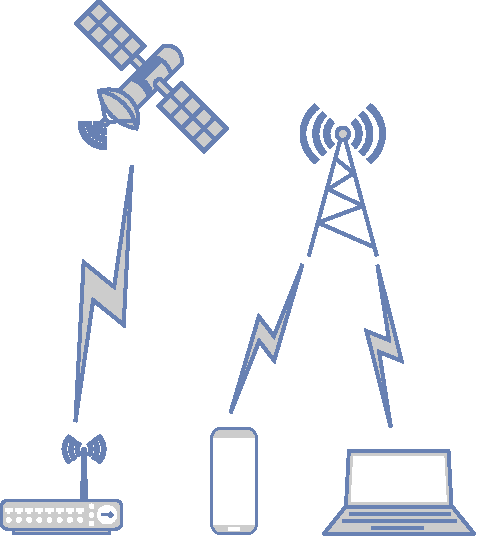
\includegraphics[
          width=\linewidth,
          height=.75\textheight,
          keepaspectratio=true,
        ]{drawiopdf/illu_telecomdig.pdf}
        \captionof{figure}{Illustration de dispositifs télécommunicants.}
      \end{center}
    \end{column}
    \begin{column}{.55\linewidth} \large
      \begin{overlayarea}{\linewidth}{.75\textheight}
        \begin{ctrlitemize}{1em}
          \item Piliers des sociétés modernes
          \item Champ englobant :
          \begin{ctrlitemize}{1em}
            \item les standards des réseaux cellulaires (\textit{Wi-Fi, 3G, 4G/LTE, 5G}),
            \item les communications en champs proches (\textit{ZigBee, NFC, Bluetooth}),
            \item les technologies de communications par satellites (\textit{DVB-S2, standards CCSDS}),
            \item et, dans le cadre de \textbf{l'Internet des objets}, les \textbf{\textcolor{red}{réseaux longues portées basses puissances (\acrshortpl{lpwan})}}.
          \end{ctrlitemize}
        \end{ctrlitemize}
      \end{overlayarea}
    \end{column}
  \end{columns}
\end{frame}

\begin{frame}{Internet des objets}
  {En anglais: \acrfull{iot}}
  \begin{columns}
    \begin{column}{.55\linewidth}
      % \small
      \begin{overlayarea}{\linewidth}{.6\textheight}
        \begin{ctrlitemize}{5pt}
          \item Croissance exponentielle ces 10 dernières années,
          \item 50 milliards d'objets connectés attendus,
        \end{ctrlitemize}

        % % \vspace{-1 ex}
        \hspace{7 em} \emph{et pourtant\dots}
        % % \vspace{-1 ex}

        \begin{ctrlitemize}{2pt}
          \item Les méthodes de transmission restent largement inspirées des précédents réseaux \dots
        \end{ctrlitemize}
      \end{overlayarea}
    \end{column}
    \begin{column}{.4\linewidth}
      \begin{center}
        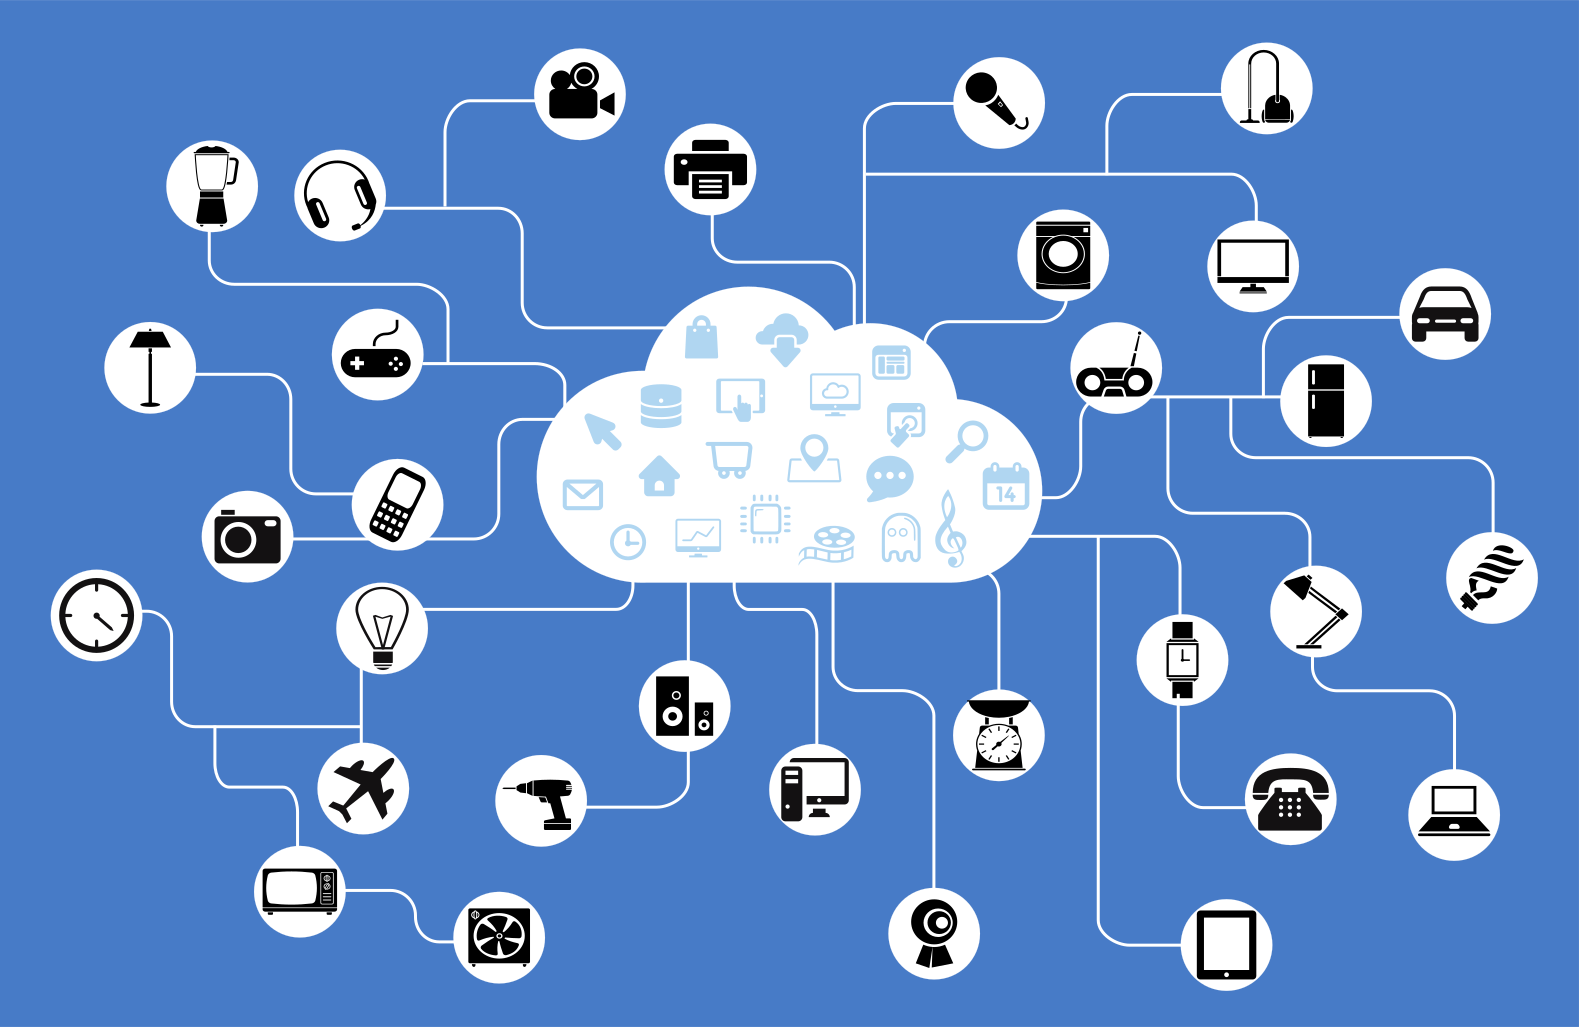
\includegraphics[
          width=\linewidth,
          height=.6\textheight,
          keepaspectratio=true
        ]{figures/svg/iot-network-wikimedia.pdf}
        \captionof{figure}{Vue d'artiste du ``cloud computing'' appliqué à de nombreux dispositifs. {\textrm{\tiny Wikimedia, CC-zero.}}}
      \end{center}
    \end{column}
  \end{columns}
  \note{
    Chez les autres, on cherche le débit ++, pas dans l'IoT !!
  }
\end{frame}

\begin{frame}{Réseaux longues portées basses puissances}
  {En anglais : \acrfullpl{lpwan}}

  \begin{columns}
    \begin{column}{.5\linewidth}
      Caractéristiques des \acrshortpl{lpwan} \cite{IEEEStandardLPWAN} :

      \begin{ctrlitemize}{5pt}
        \item Communications longues portées (dizaines de kilomètres).
        \item Permettent le déploiement massif d'objets connectés.
        \item Quantité de données à transmettre et donc débits requis plus faibles.
        \item Topologie typique : des nœud-capteurs bas-coûts et des stations de base haute-performances.
      \end{ctrlitemize}
    \end{column}
    \begin{column}{.5\linewidth}
      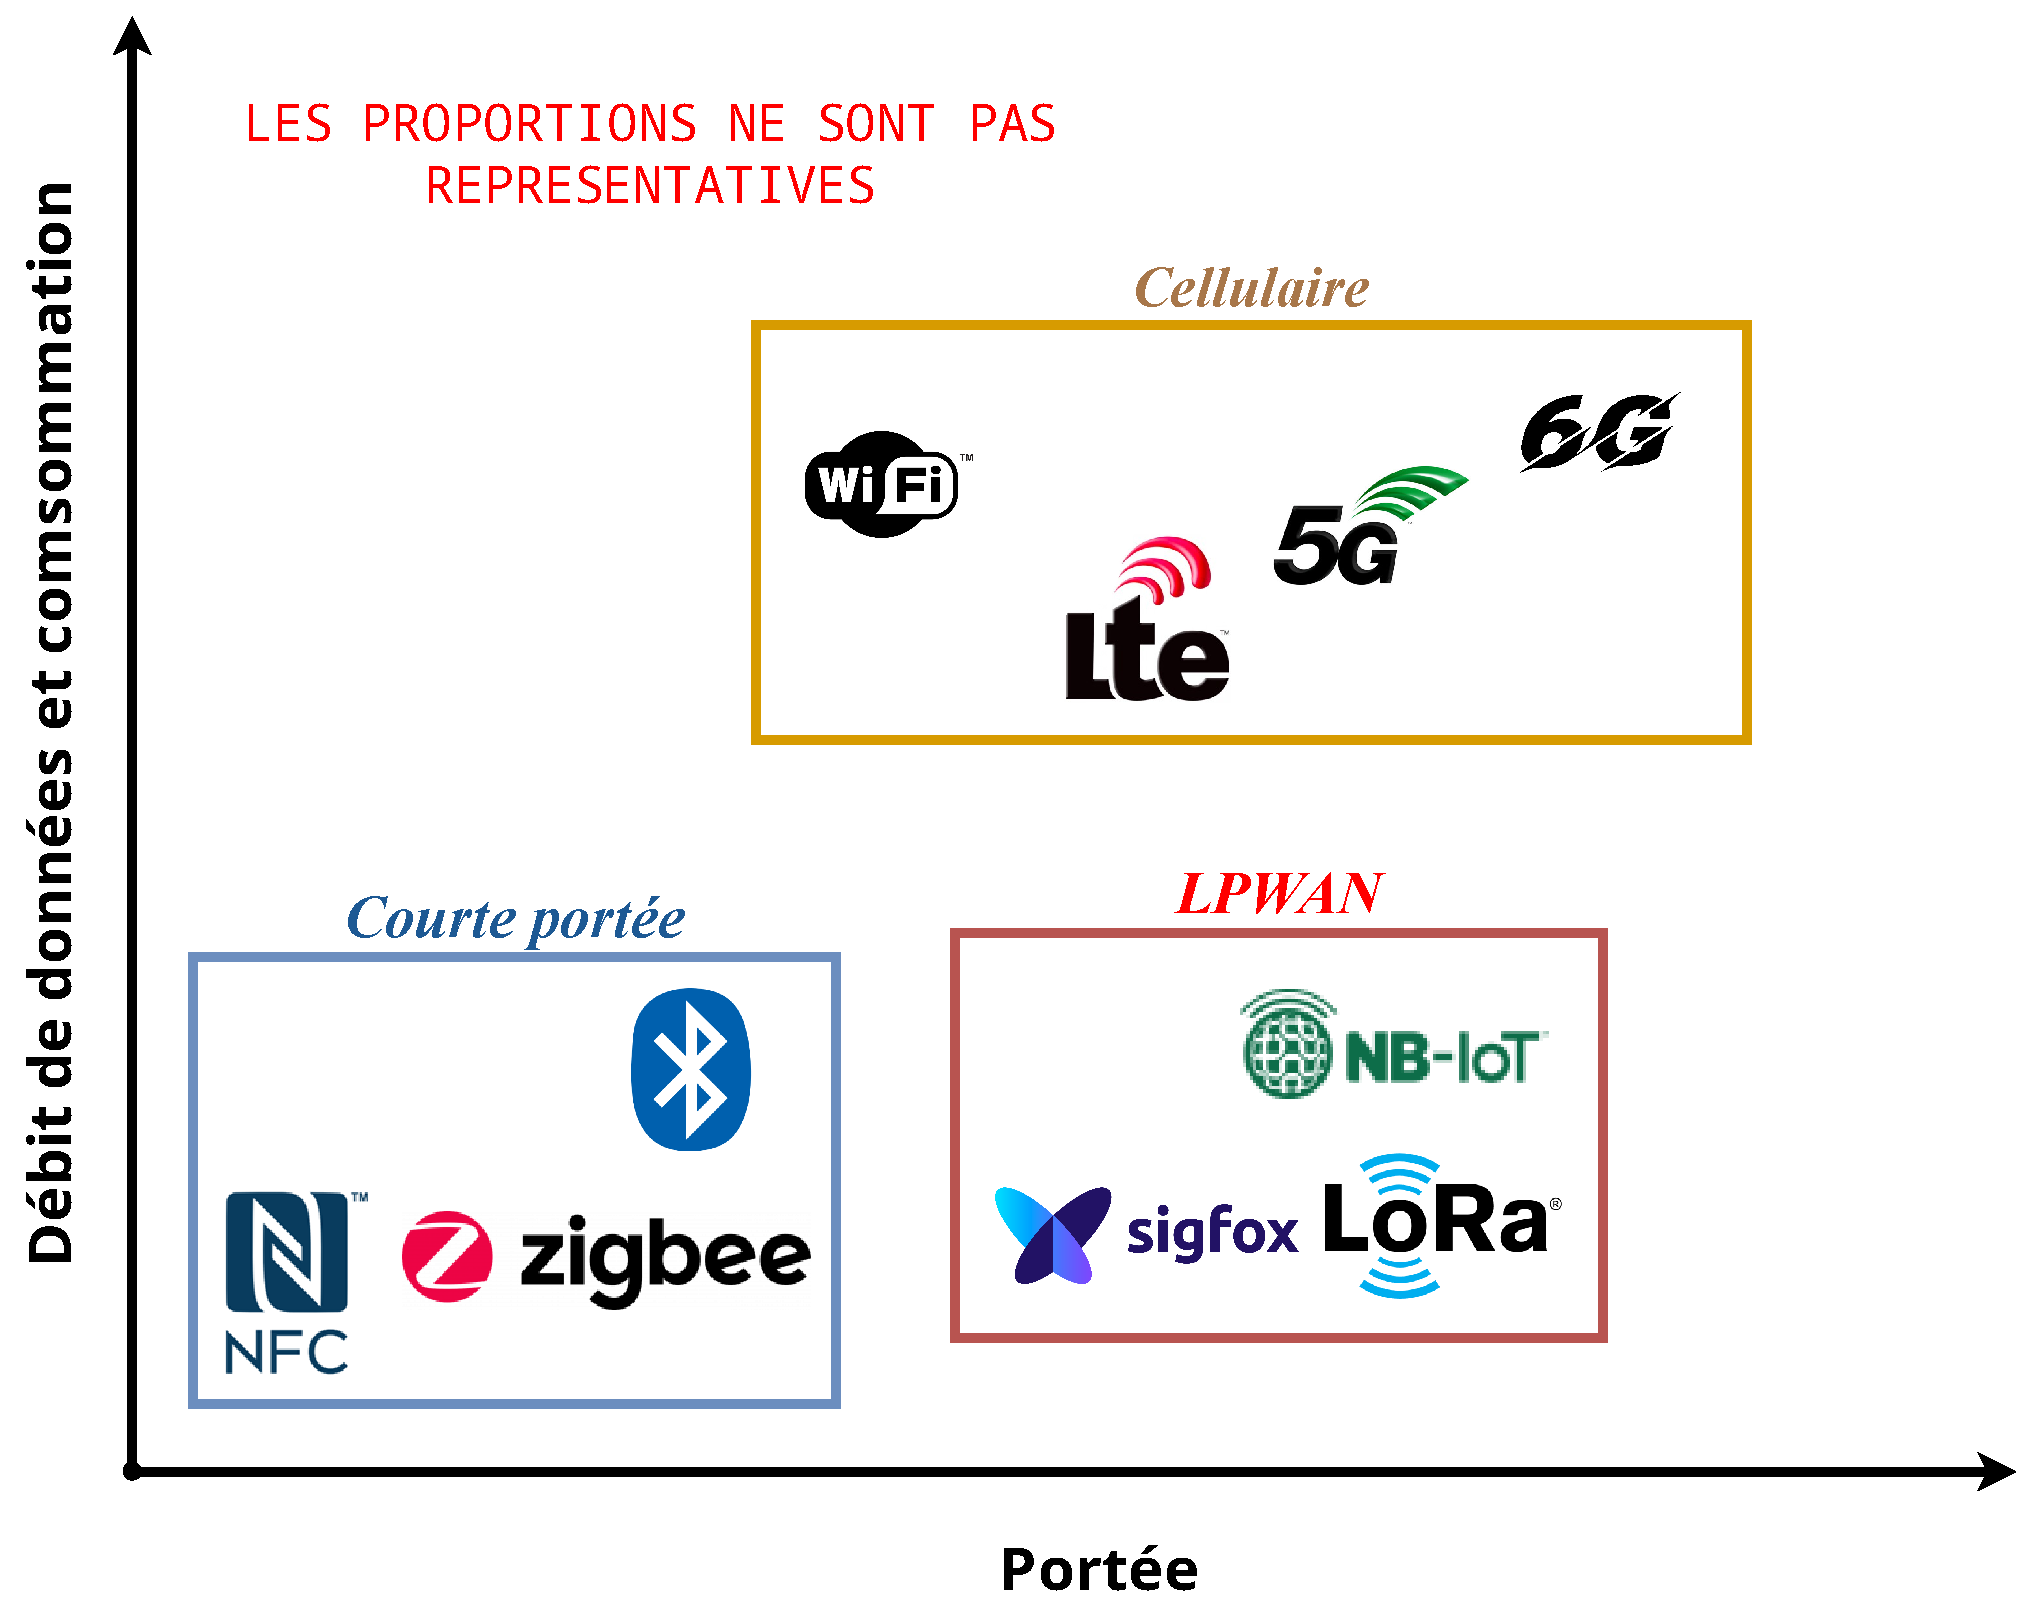
\includegraphics[width=\linewidth, height=.65\textheight, keepaspectratio=true]{figures/drawiopdf/lpwan_and_co.pdf}
      \captionof{figure}{Positionnement des technologies \acrshort{lpwan} SigFox, LoRa et NB-IoT par rapport aux réseaux cellulaires ou courtes portées \cite{sinhaSurveyLPWATechnology2017}.}
    \end{column}
  \end{columns}
  \blfootnotetext{\textcite{IEEEStandardLPWAN, sinhaSurveyLPWATechnology2017}}
  \note{
    \begin{itemize}
      \item Portée (parfois comparable au cellulaire)
      \item MAIS but déploiement massif
      \item Petit packets
      \item basse conso'
      \item petits objets, grosse station
    \end{itemize}
  }
\end{frame}

\begin{frame}{\acrshortpl{lpwan} : trois exemples}

  % Le \acrshortpl{lpwan} ont connu un fort développement durant la dernière décennie, de nombreux standards ont vu le jour\cite{goursaudDedicatedNetworksIoT2015, sinhaSurveyLPWATechnology2017}.%

  \begin{columns}
    \begin{column}{.5\linewidth} \centering
      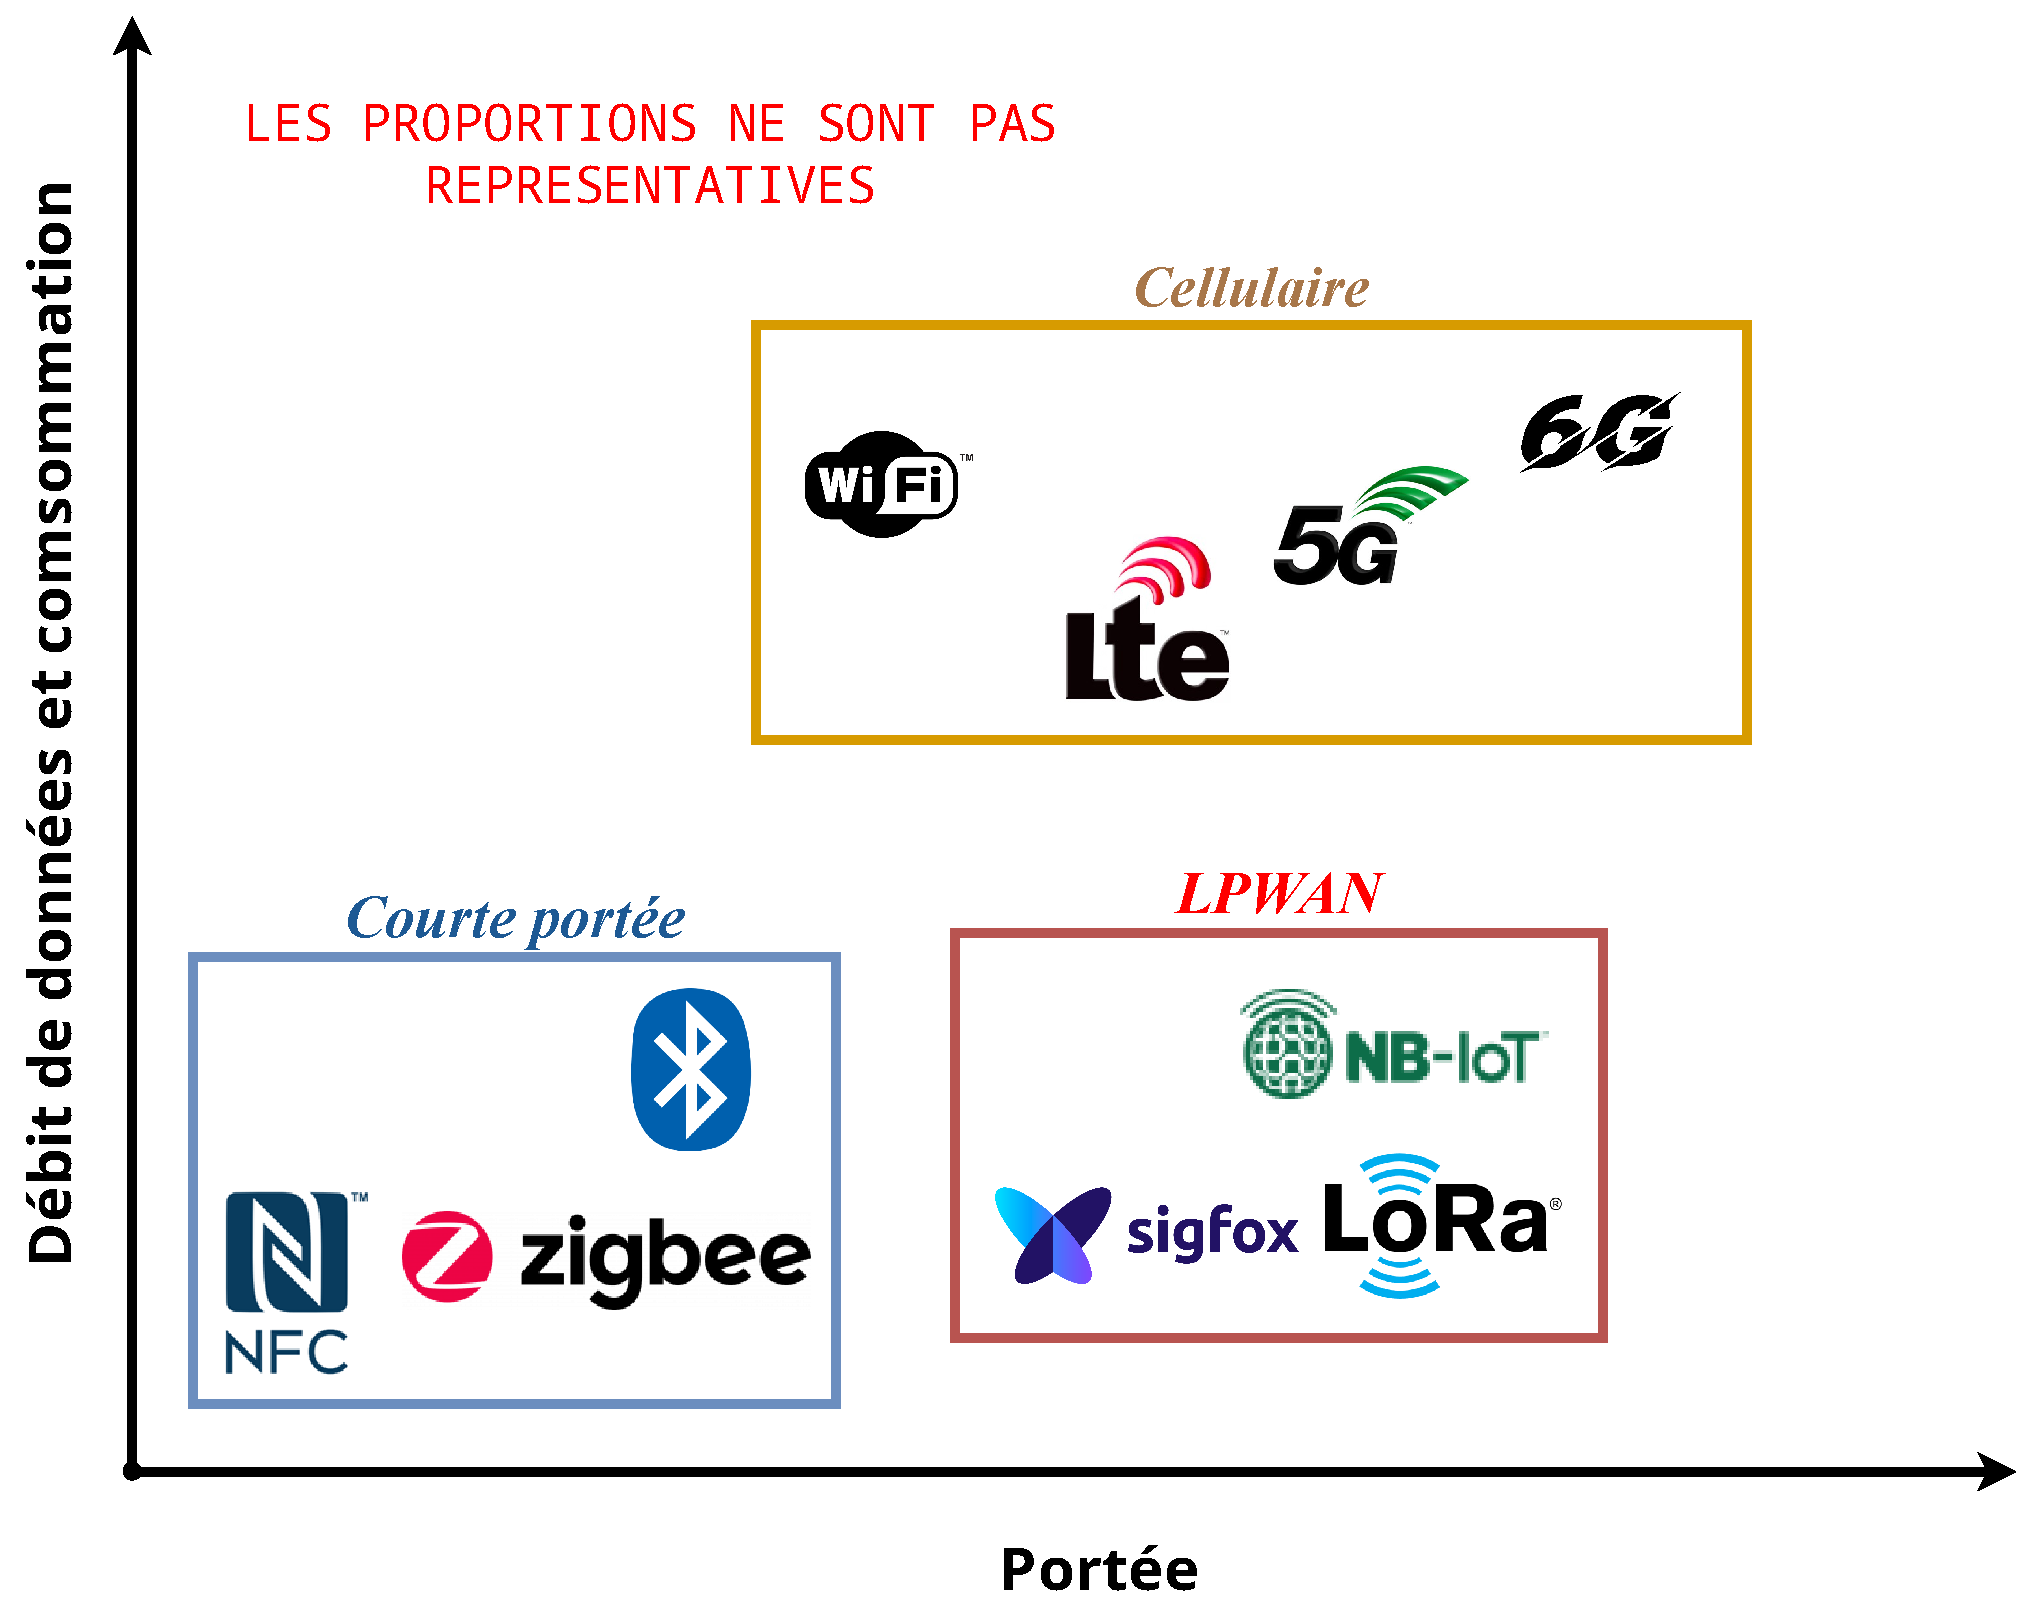
\includegraphics[width=\linewidth, height=.65\textheight, keepaspectratio=true]{figures/drawiopdf/lpwan_and_co.pdf}
      \captionof{figure}{Positionnement des technologies \acrshort{lpwan} SigFox, LoRa et NB-IoT comparé à celles des réseaux cellulaires ou courtes portées \cite{sinhaSurveyLPWATechnology2017}.}
    \end{column}

    \begin{column}{.5\linewidth} \centering
      \ra{1.3}
      % \begin{noindent}
    \begin{tabular}[t]{@{}c@{\phantom{XX}}c@{\phantom{X}}c@{\phantom{X}}c@{}}
      \toprule
                                & \textbf{SigFox} & \textbf{LoRa} & \textbf{NB-IoT} \\ \midrule
      % \textbf{Modulation}    & \acrshort{bpsk}   & \acrshort{css}    & \acrshort{qpsk}     \\ 
      % \textbf{Fréquence centrale}
      %                        & $868$ MHz         & $868$ MHz         & bandes LTE          \\
      % \textbf{Largeur de bande}
      %                        & $0.1$ kHz         & $125$/$250$ kHz   & $200$ kHz           \\
      \coltab{\textbf{Débit max}\\\textit{(kb/s)}} 
                                & \textcolor{red}{$0.1$} & \textcolor{RoyalBlue2}{$50$}  & \textcolor{Chartreuse3}{$200$}      \\
      % \textbf{Taille max de la charge utile}
      %                        & $96$ bits         & $1944$ bits       & $12.8$ kilobits     \\
      \coltab{\textbf{Portée max}\\\textit{(km)}} 
                                & \textcolor{Chartreuse3}{$40$}   & \textcolor{RoyalBlue2}{$20$} & \textcolor{red}{$10$}        \\
      \textbf{Robustesse}       & \textcolor{Chartreuse3}{++}     & \textcolor{Chartreuse3}{++}   & \textcolor{red}{-}           \\
      % \textbf{Code(s) correcteur(s) d'erreur}
      %                        & aucun             & codes de Hamming  & codes modernes      \\
      \bottomrule
    \end{tabular}
    % \end{noindent}
      \captionof{table}{Aperçu des caractéristiques de trois technologies dans les \acrshortpl{lpwan}, SigFox, LoRa et NB-IoT \cite{goursaudDedicatedNetworksIoT2015}.}
      \ra{1}
    \end{column}
  \end{columns}
  \blfootnotetext{\textcite{goursaudDedicatedNetworksIoT2015, sinhaSurveyLPWATechnology2017}}
\end{frame}

\begin{frame}{Chaine de communication classique}{} \centering \vspace{-1em}

  \begin{columns}
    \begin{column}{.15\linewidth} \centering
      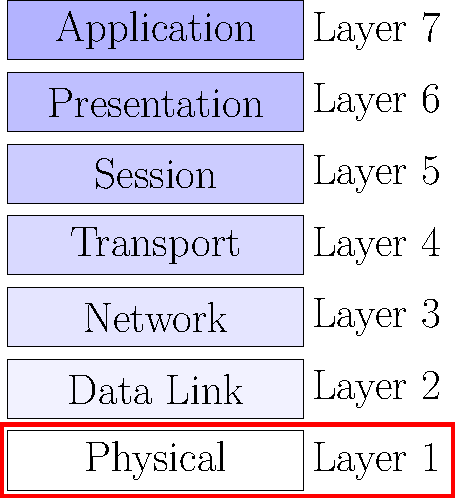
\includegraphics[width=\linewidth]{figures/tikzpicture/osi_layers_stdl.pdf}
      \captionof{figure}{Modèle OSI (\textit{Open Systems Interconnection}).}
    \end{column}
    \begin{column}{.6\linewidth}
      \only<1>{
        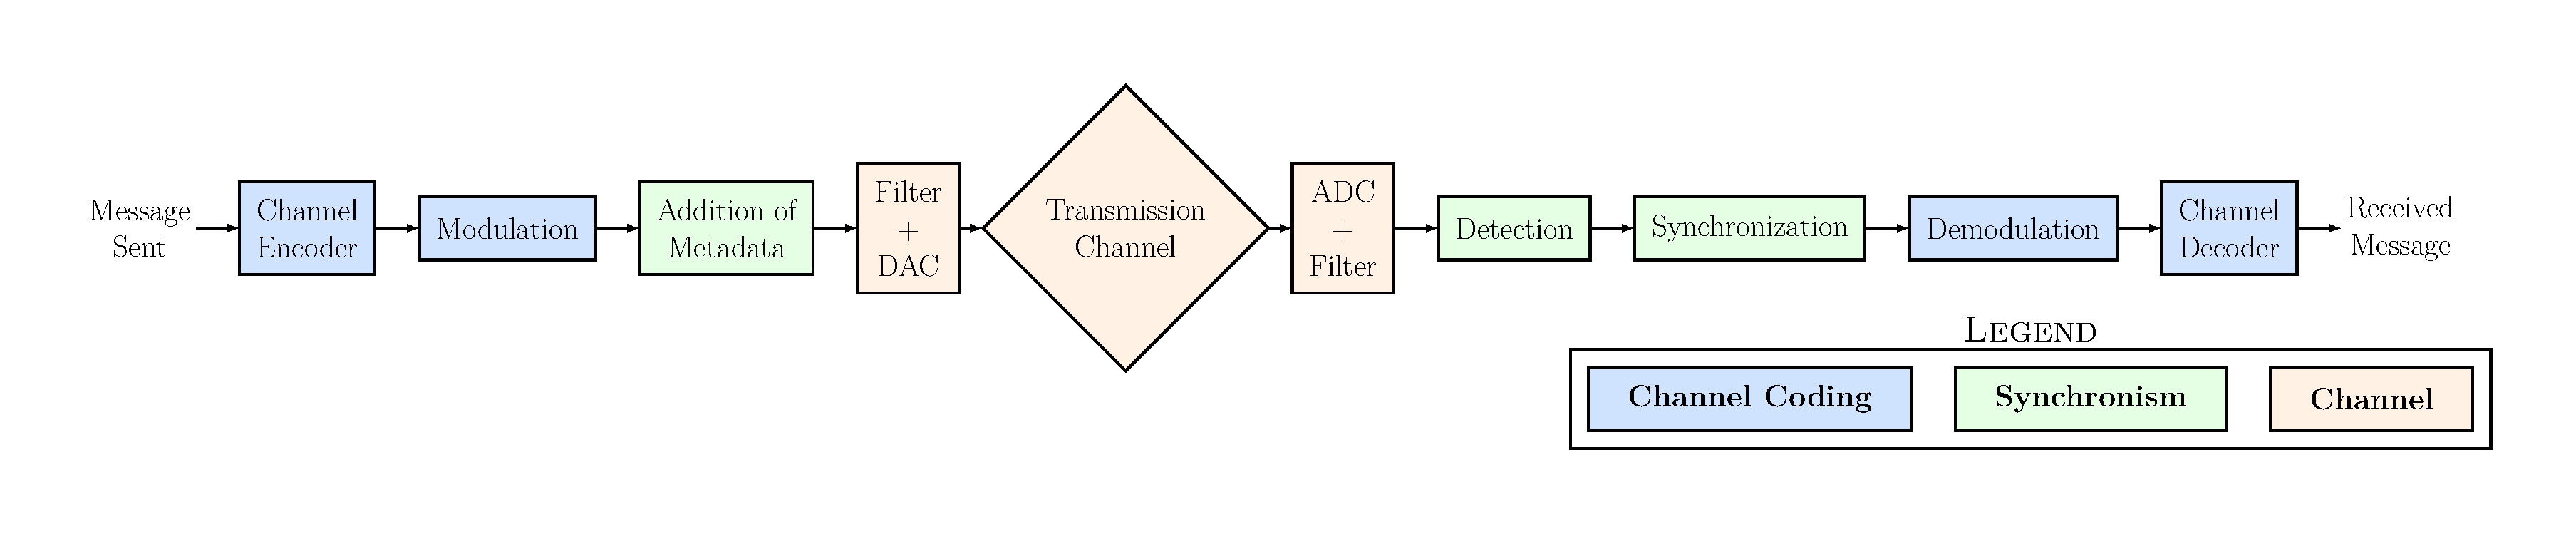
\includegraphics[width=\linewidth, height=.9\textheight, keepaspectratio=true]{tikzpicture/async_comm_chain_stdl.pdf}
      }
      \only<2>{
        \includegraphics[width=\linewidth, height=.9\textheight, keepaspectratio=true]{tikzpicture/async_comm_chain_stdl-2.pdf}
      }
    \end{column}
  \end{columns}

  \vspace{-1em}

  \begin{columns} \small
    \begin{column}{.45\linewidth}
      \begin{itemize}
        \item [CNA :] Convertisseur Numérique Analogique
      \end{itemize}
    \end{column}
    \begin{column}{.45\linewidth}
      \begin{itemize}
        \item [CAN :] Convertisseur Analogique Numérique
      \end{itemize}
    \end{column}
  \end{columns}
  \note{
    Décrit la chaine puis\\
    Cadre thèse ->\\
    Cadre présentation. 
  }
\end{frame}

\begin{frame}{Problème des préambules}
  % \begin{overlayarea}{\linewidth}{.05\textheight}
  % \end{overlayarea}
  \begin{columns}
    \begin{column}{.155\linewidth}
      \hfill
    \end{column}
    \begin{column}{.69\linewidth}
      \begin{overlayarea}{\linewidth}{.45\textheight}
        \only<1,2>{
          \includegraphics[
            width=\linewidth,
            keepaspectratio=true
          ]{figures/tikzpicture/joint_frame_tikz_bare.pdf}
        }
        \only<2>{
          Les \emph{métadonnées} de détection et synchronisation représentent parfois jusqu'à  50\% de la consommation de ressources \cite{durisiMassiveUltrareliableLowLatency2016, polyanskiyAsynchronousCommunicationExact2013}.
        }
        \only<3>{
          \includegraphics[
            width=\linewidth,
            keepaspectratio=true
          ]{figures/tikzpicture/joint_frame_tikz.pdf}
        }
      \end{overlayarea}
    \end{column}
    \begin{column}{.155\linewidth}
      \hfill
    \end{column}
  \end{columns}

  \begin{overlayarea}{\linewidth}{.4\textheight}
    \only<1>{
      \includegraphics[width=\linewidth]{figures/tikzpicture/joint_frame_tikz_leg.pdf}
    }
    \only<2->{ \centering
      \includegraphics[width=\linewidth]{figures/tikzpicture/joint_frame_tikz_leg-2.pdf}
    }
  \end{overlayarea}
  \blfootnote{\textcite{durisiMassiveUltrareliableLowLatency2016, polyanskiyAsynchronousCommunicationExact2013}}
  \note{
    \begin{enumerate}
      \item Classiquement le paquet, c'est ça
      \item Mais dans l'iot, pas ouf !! (50\% ...)
      \item Peut-on se passer de ces métadonnées, et rester temps réel ?!
      \item PB Syncro temps fréquence, pas d'info à priori !
    \end{enumerate}
  }
\end{frame}

\end{document}
